\chapter{Umsetzung und Implementation}
\label{chap:implementation}

%%%%%%%%%%%%%%%%%%%%%%%%%%%%%%%%%%%%%%%%%%%%%%%%%%%%%%%%%%%%
\section{Ansatz zur Positionsbestimmung}
\label{sec:implementation:positioning}
%%%%%%%%%%%%%%%%%%%%%%%%%%%%%%%%%%%%%%%%%%%%%%%%%%%%%%%%%%%% 
Bei der Positionsbestimmung geht es um die Bestimmung des aktuellen Ortes in Echtzeit und das auf bis zu 10cm genau. Bei der Positionsangabe handelt es sich hier um eine zweidimensionale Position, da dies für unsere Zwecke ausreicht.

Bei der Positionsbestimmung wurden zwei verschiedene Ansätze untersucht. Zum einen die Trilateration, welche eine Positionierung mittels Entfernungen zu verschiedenen Fixpunkten ermöglicht und zum Anderen die Positionierung mittels Fingerprinting, welches eine Datenbank mit sogenannten Fingerprints, also vorher aufgezeichneten Messwerten und damit verbundenen Positionsdaten, voraussetzt und darüber die aktuelle Position bestimmt.

Die Positionsbestimmung soll dabei in einem 2D-Raum erfolgen, da die Höhe vernachlässigt werden kann. In der realen Welt kann die Höhe ebenfalls vernachlässigt werden, da dort Stockwerke meist einen deutlichen Höhenunterschied aufweisen, sodass dieser über andere Faktoren eindeutig bestimmt werden kann.


%%%%%%%%%%%%%%%%%%%%%%%%%%%%%%%%%%%%%%%%%%%%%%%%%%%%%%%%%%%%
\section{Trilateration}
\label{sec:implementation:trilateration}
%%%%%%%%%%%%%%%%%%%%%%%%%%%%%%%%%%%%%%%%%%%%%%%%%%%%%%%%%%%%
Die Trilateration ist eine Methode zur Bestimmung der aktuellen Position. Im Gegensatz zur Triangulation, welche die Position anhand der Winkelgrößen zwischen verschiedenen Fixpunkten bestimmt, wird bei der Trilateration die Position durch die Abstände zu den Fixpunkten bestimmt. 

Bei der Trilateration wird der Abstand zu einem Fixpunkt genutzt, um die Position des Objektes zu bestimmen. Das Objekt muss dabei auf einer Kreisbahn um den Fixpunkt liegen, welche den Radius des zuvor bestimmten Abstand besitzt. Um nun einen genauen Standpunkt zu bestimmen, sind mindestens drei Fixpunkte und die dazugehörige Abstände nötig, da so im zweidimensionalem Raum ein eindeutiger Schnittpunkt entsteht.

\begin{figure}[htb!]
	\centering
	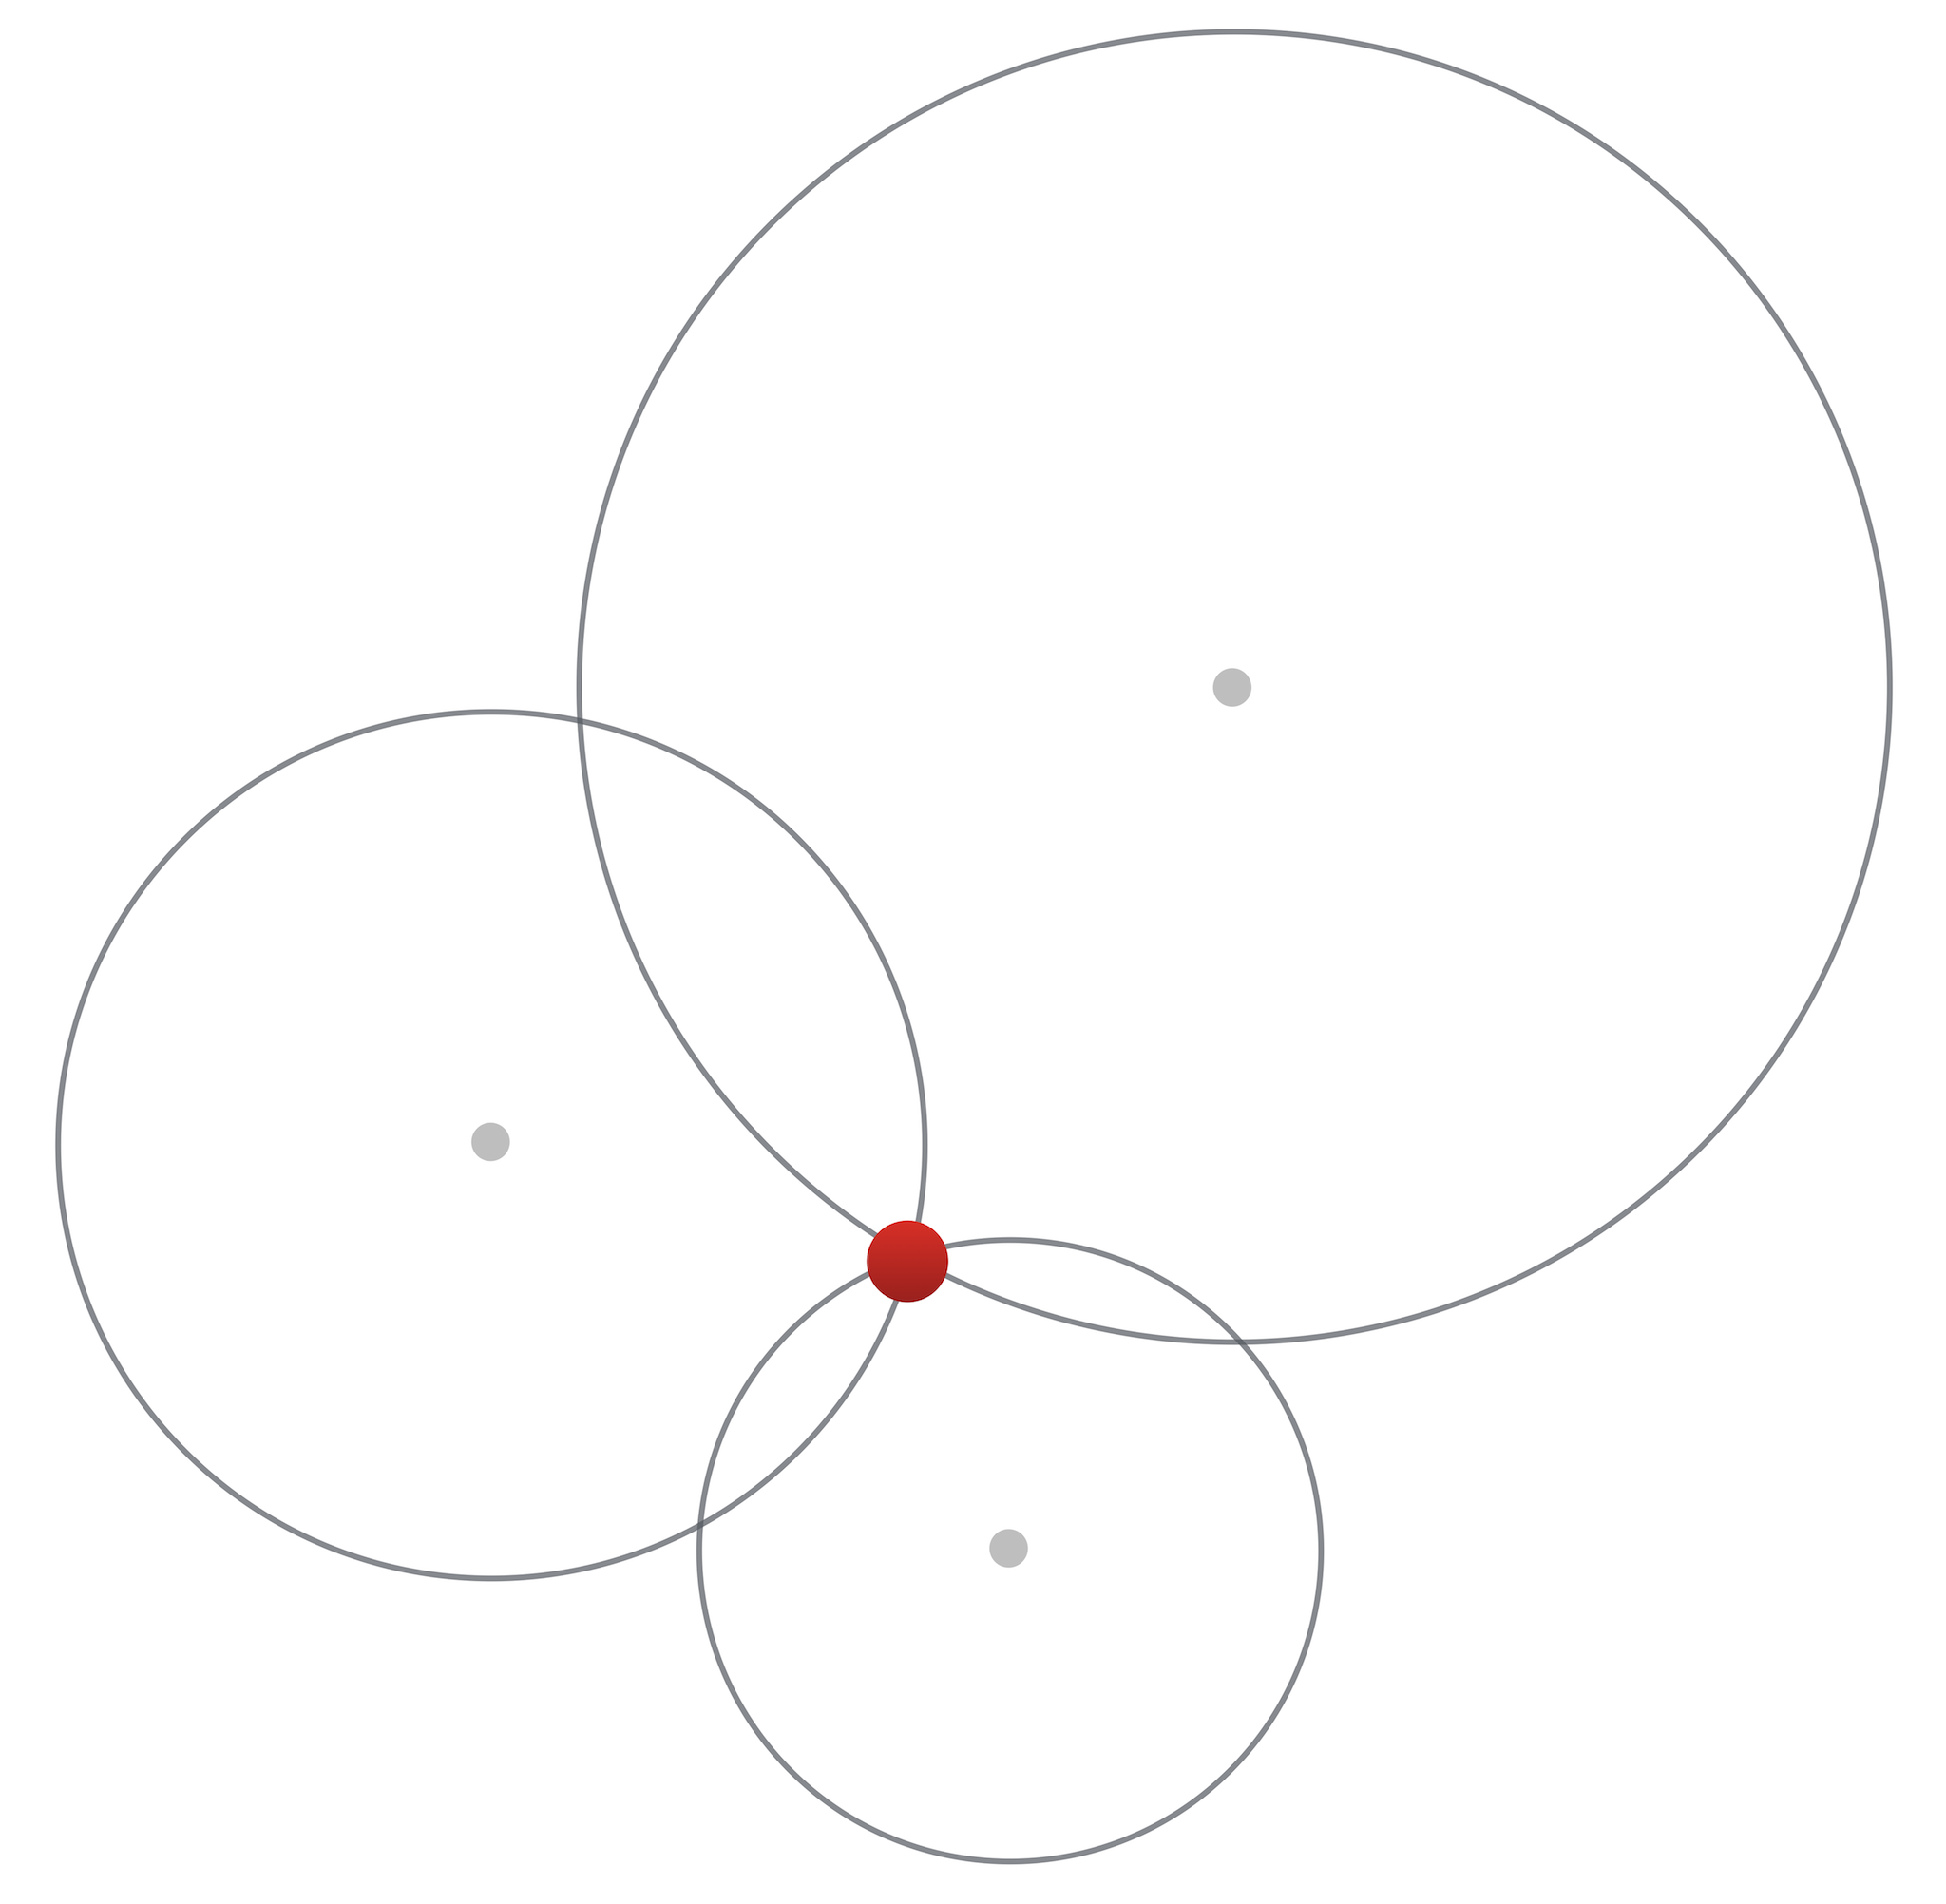
\includegraphics[scale=1.5]{trilateration}
	\caption{Funktionsprinzip der Trilateration}
	\label{trilateration-accurate}
\end{figure}

In Abbildung \ref{trilatertion-accurate} sieht man dabei die Funktionsweise der Trilateration bei genauer Abstandsbestimmung. In realen Messungen und Positionsbestimmungen ist es jedoch nicht möglich genaue Abstände zu bestimmen, da es immer zu Messungenauigkeiten kommen kann.
Bei solchen ungenauen Messungen ist es nun nicht mehr möglich einen genauen Schnittpunkt zu finden. 

Um diese Ungenauigkeit auszugleichen wird das Verfahren entsprechend angepasst. Dabei werden Geraden durch die Schnittpunkte der einzelnen Umkreise gelegt. Dadurch entsteht zwischen den Geraden ein neuer Schnittpunkt, welcher die aktuelle Position repräsentiert. Dieses Verfahren wird in Abbildung \ref{trilateration-inaccurate} dargestellt.

\begin{figure}[htb!]
		\centering
	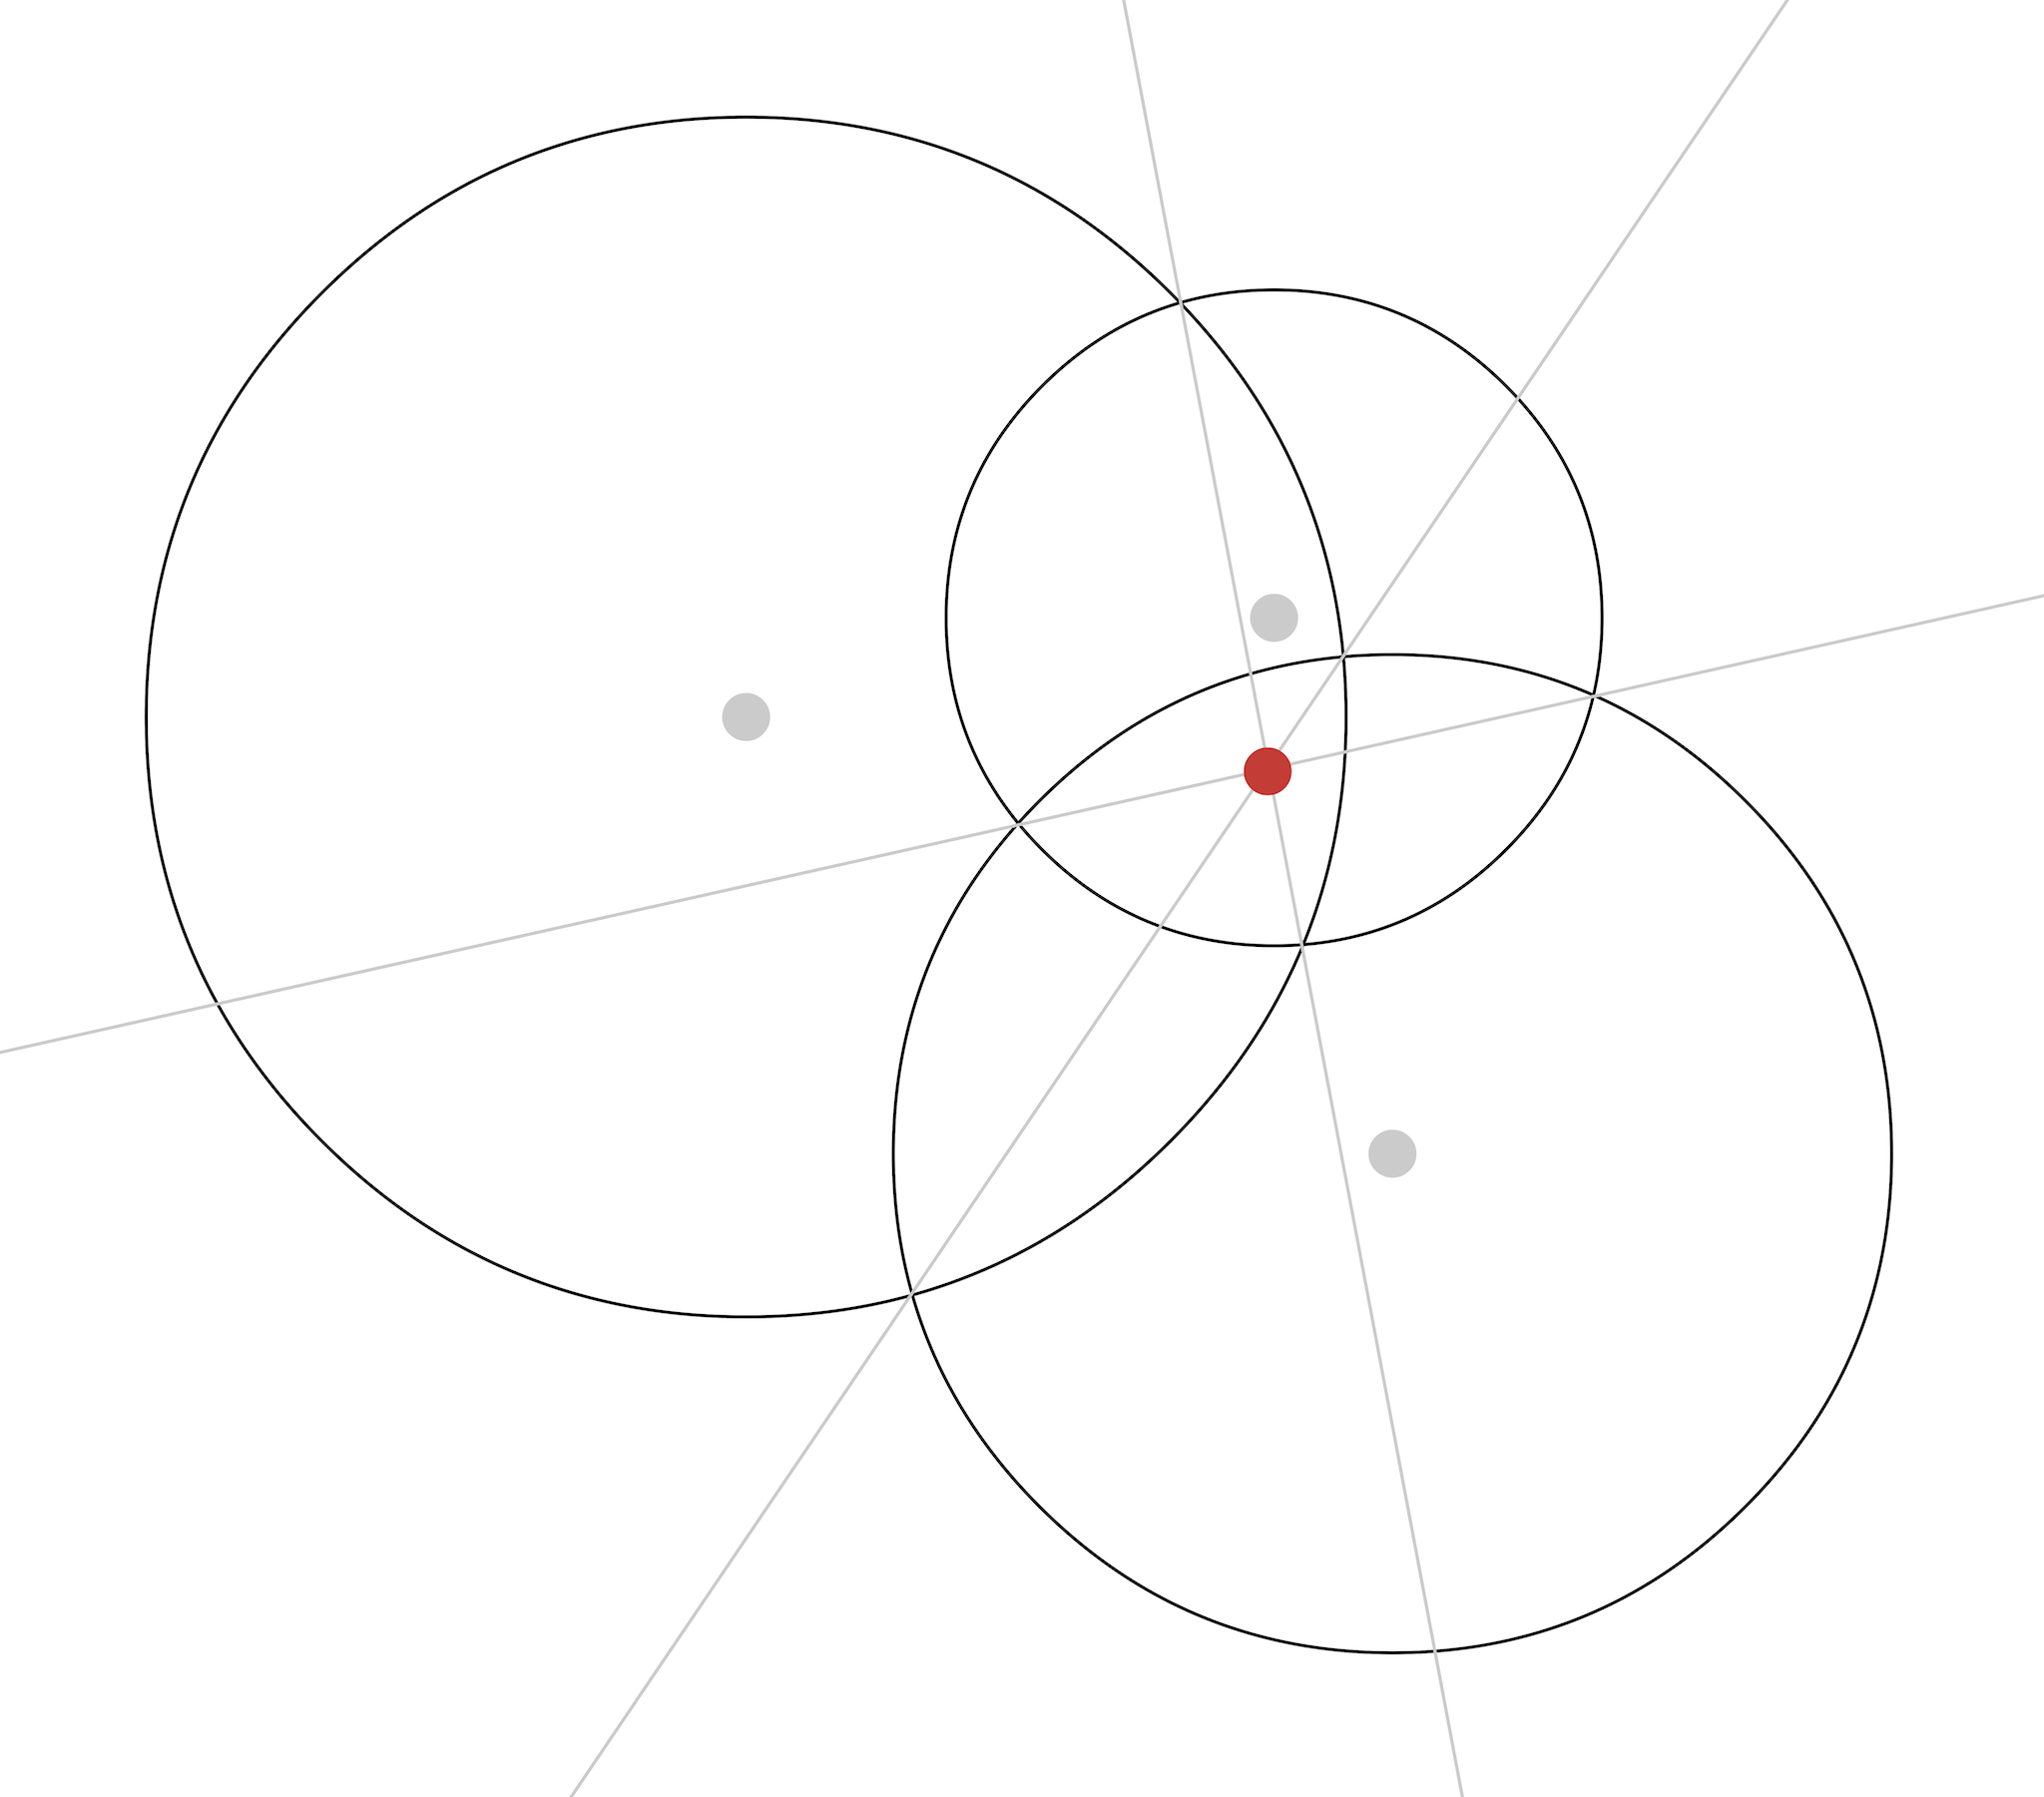
\includegraphics[scale=1.5]{trilateration-inaccurate}
	\caption{Trilateration bei ungenauen Abständen zu den Fixpunkten}
	\label{trilateration-inaccurate}
\end{figure}

Damit ist es möglich auftretende Ungenauigkeiten zu kompensieren und trotzdem eine genaue Positionbestimmung durchzuführen.

Bei der genutzten iBeacons beziehungsweise Bluetooth-Technologie ist eine genaue Entfernungsangabe jedoch nicht vorgesehen, wodurch das Verfahren der Trilateration nicht direkt angewand werden kann. Dafür muss zunächst ein Ersatzindikator für die Entfernungsmessung bestimmt werden.
Bei der Bluetooth-Technologie bietet sich dafür die Signalstärke an.
Dabei wird die Tatsache genutzt, dass die Signalstärke mit zunehmendem Abstand sinkt und man somit aus der aktuellen Signalstärke auch die aktuelle Entfernung bestimmen kann. 
Das Verhältnis zwischen Entfernung und Signalstärke bei elektromagnetischen Wellen wird durch das Abstandsgesetz beschrieben, welches besagt, das die Signalstärke quadratisch zum Abstand abnimmt.

\begin{equation}
	\text{\emph{Signalstärke}} = \text{\emph{Ausgangssignalstärke}}/\text{\emph{Entfernung}}^2
\end{equation}

Diese Annahme mag bei freien Flächen korrekt sein, in Innenräumen kommen jedoch weitere Faktoren hinzu. 
Durch Wände und Hindernisse im Raum, wie zum Beispiel Schränke, Regale, usw., kommt es dort zu einer Dämpfung des Signals, wodurch die Signalstärke beeinflusst wird. Des Weiteren kann es in Innenräumen auch zu Streuung und Reflexionen kommen, welche das Signal zusätzlich verfälschen.

Diese Annanahme bestätigt sich auch bei den Messungen. Diese zeigen, dass die gemessene Signalstärke nicht, wie angenommen, mit der Entfernung stetig abnimmt, sondern sehr stark schwankt, wodurch keine genaue Entfernungsbestimmung durchgeführt werden kann.

Die Methode der Trilateration wurde auf Grund der fehlenden Genauigkeit verworfen. 

%%%%%%%%%%%%%%%%%%%%%%%%%%%%%%%%%%%%%%%%%%%%%%%%%%%%%%%%%%%%
\section{Fingerprinting}
\label{sec:implementation:fingerprinting}
%%%%%%%%%%%%%%%%%%%%%%%%%%%%%%%%%%%%%%%%%%%%%%%%%%%%%%%%%%%%
Das Fingerprinting ist ein Verfahren der Positionsbestimmung auf der Grundlage von zuvor erhobenen Messwerten, den sogenannten Fingerprints.
Die Funktionsweise des Fingerprintings unterscheidet sich grundlegend von der Methode der Trilateration, da hierbei keine direkte Berechnung der Position über Entfernungsgrößen geschieht, sondern die Positionierung über, in einer Datenbank abgelegten Erfahrungswerten geschieht.

Um dieses Verfahren umzusetzen muss der Messraum, in welchem die Positionierung statt finden soll, zunächst in ein Gitternetz eingeteilt werden, wobei jede Zelle des Gitters eine mögliche Position im Raum repräsentiert. Die Größe dieser Zellen ist prinzipiell frei wählbar, wird jedoch im wesentlichen durch zwei Faktoren bestimmt. 
Zum einen die gewünschte Genauigkeit. Da jede Zelle eine mögliche Position repräsentiert, wird durch die Größe der Zellen auch die Genauigkeit der Position bestimmt. Daraus ergibt sich das die Genauigkeit zunimmt, wenn die Zellengröße verkleinert wird.
Der zweite Faktor bei der Wahl der Zellengröße, ist die eindeutige Bestimmung der Zelle. Dies ist darauf zurückzuführen, dass bei kleineren Zellen die Differenzen zwischen den einzelnen Zellen ebenfalls abnehmen. Um nun eine genaue Bestimmung der Zelle zu ermöglichen, sollte jede Zelle so groß gewählt werden, dass dies noch möglich ist.

Daher sollte die Zellengröße so gewählt werden, dass eine gute Unterscheidbarkeit zwischen den einzelnen Zellen gewährleistet ist, hinzu jedoch eine möglichst geanue Positionsbestimmung erzielt werden kann.


Das Fingerprinting besteht im Wesentlichen aus zwei Phase.

Die erste Phase ist die sogenannte \emph{Trainingsphase}. Dabei werden die sogenannten \emph{Fingerprints} gesammelt, welche letzlich zur Positionsbestimmung genutzt werden. 
In der Trainingsphase werden daher, für jede Zelle unseres Messraumes eine Reihe von Fingerprints gesammelt. Die Anzahl der Fingerprints sollte dabei relativ groß sein, sodass Messfehler kompensiert werden können. 
Ein Fingerprint kann sich dabei aus verschiedenen Daten zusammensetzen. 
In diesem Fall besteht ein Fingerprint aus der aktuellen Zellennummer beziehungsweise der Zellenkoordinate, einem Zeitstempel mit aktuellem Datum und der Uhrzeit und den Signalstärken zu den verschiedenen, in Reichweite befindlichen Sendestationen, welches in diesem Fall die iBeacons sind.

Die Sammlung der Fingerprints muss für jede Zelle geschehen und macht die Trainingsphase daher sehr zeitaufwendig. 

Die der zweiten Phase, auch \emph{Onlinephase} genannt, werden die zuvor gesammelten Informationen verwendet um die aktuelle Position zu bestimmen. 
Dafür werden die gesammelten Fingerprints mit den aktuell gemessenen Signalstärken verglichen. Wenn eine Übereinstimmung gefunden wird, wird die Position des passenden Fingerprints als aktuelle Position angenommen.

\todo{Einfügen von Zeichnung welche Zellen und Fingerprints verdeutlicht}

%%%%%%%%%%%%%%%%%%%%%%%%%%%%%%%%%%%%%%%%%%%%%%%%%%%%%%%%%%%%
\subsection{Positionsbestimmung}
\label{sec:implementation:fingerprinting:positioning}
%%%%%%%%%%%%%%%%%%%%%%%%%%%%%%%%%%%%%%%%%%%%%%%%%%%%%%%%%%%%
Bei der Positionsbestimmung mittels Fingerprinting gibt es verschiedene Ansätze.
Das erste Verfahren vergleicht alle Fingerprints in der Datenbank mit den aktuellen Messwerten und bestimmt damit die aktuelle Position.
Eine weitere Möglichkeit besteht darin, den Durchschnittswert der Fingerprints zu bilden um diesen dann mit den aktuellen Werten zu vergleichen.
Die letzte untersuchte Möglichkeit ist die der Wahrscheinlichkeitsverteilung der Werte. Hier wird über die Wahrscheinlichkeitswerte der einzelnen Messwerte die aktuelle Position bestimmt.

%%%%%%%%%%%%%%%%%%%%%%%%%%%%%%%%%%%%%%%%%%%%%%%%%%%%%%%%%%%%
\subsection{Einfache Positionsbestimmung}
\label{sec:implementation:fingerprinting:positioning:naiv}
%%%%%%%%%%%%%%%%%%%%%%%%%%%%%%%%%%%%%%%%%%%%%%%%%%%%%%%%%%%%
Bei der einfachen und naiven Bestimmung der aktuellen Position, werden alle zuvor gesammelten Fingerprints mit den aktuell gemessenen Signalstärken verglichen. Dies führt dazu, dass bei größeren Fingerprint-Datenbanken auch die Rechenzeit und der Energieverbrauch steigt. 

Bei dem Vergleich der Messwerte mit den gespeicherten Fingerprints wird das Nearest-Neighbor-Verfahren verwendet. Dabei werden sowohl die aktuellen Messwerte, als auch die Fingerprints als Vektoren aus den Signalstärken zusammengefasst und aus diesen Vektoren wird die jeweilige Entfernung der beiden Werte berechnet.

\begin{equation}
	\begin{pmatrix}
		RSSI1 \\
		RSSI2 \\
		RSSI3 \\
		...
	\end{pmatrix}
	\begin{pmatrix}
		Measured RSSI1 \\
		Measured RSSI2 \\
		Measured RSSI3 \\
		...
	\end{pmatrix}
\end{equation}

